\documentclass[12pt,twocolumn]{article}

% Page dimensions
\setlength{\hoffset}{-0.4in}
\setlength{\voffset}{-0.5in}
%\setlength{\headsep}{-0.2in}

\setlength{\oddsidemargin}{0in}
\setlength{\textwidth}{7.4in}
\setlength{\textheight}{8.5in}

\setlength{\columnsep}{0.3in}

% Packages
\usepackage{fancyhdr}
\usepackage{lastpage}
\usepackage{abstract}
\usepackage{amsmath, amssymb} 
\usepackage{epsfig}
\usepackage{subcaption} 
\usepackage[english]{alg}
\usepackage[usenames,dvipsnames]{color}
\usepackage{empheq}
%\usepackage[hidelinks]{hyperref}
\usepackage{hyperref}
\usepackage{sectsty}

\usepackage{morefloats}

% Packages for notes, testing, etc.
\usepackage{todonotes}
\usepackage[inline]{showlabels}

\showlabels[\color{blue}]{cite}
\showlabels[\color{blue}]{ref}

%% ============================================================

% Macros
\newcommand{\CHRONO}{{\sffamily{{Chrono}}}}
\newcommand{\ChronoFEA}{{\sffamily{Chrono}}::FEA}
\newcommand{\ChronoVehicle}{{\sffamily{Chrono}}::Vehicle}
\newcommand{\ChronoFSI}{{\sffamily{Chrono}}::FSI}
\newcommand{\ChronoGranular}{{\sffamily{Chrono}}::Granular}
\newcommand{\ChronoParallel}{{\sffamily{Chrono}}::Parallel}
\newcommand{\ChronoDistributed}{{\sffamily{Chrono}}::Distributed}
\newcommand{\ChronoOpenGL}{{\sffamily{Chrono}}::OpenGL}

%% ============================================================

% Styles

\definecolor{my-gray}{gray}{0.4}

% First page header
\fancypagestyle{firststyle} {
	\lhead{}
	\rhead{
	\footnotesize
	\textbf{2017 NDIA GROUND VEHICLE SYSTEMS ENGINEERING AND TECHNOLOGY SYMPOSIUM}\\
	\textbf{\sc Modeling \& Simulation, Testing and Validation (MSTV) Technical Session}\\
	\textbf{\sc August 8-10, 2017 -- Novi, Michigan}	
	}
	\chead{}
	%
	\lfoot{}
	\cfoot{}
	\rfoot{}
}

% All other pages (header and footer)
\pagestyle{fancy}
\fancyhf{}
\rhead{
	\color{my-gray}
	\footnotesize Proceedings of the 2017 Ground Vehicle Systems Engineering and Technology Symposium (GVSETS)
	}
\cfoot{
	\color{my-gray}
	\footnotesize
	{\FooterTitle}\\
	Page \thepage~of~\pageref{LastPage}
}

\renewcommand{\headrulewidth}{0pt}

% Font and styles for sections
\allsectionsfont{\fontsize{12}{15}\selectfont}

\renewcommand{\abstractname}{ABSTRACT}
\renewcommand{\refname}{REFERENCES}

%% ============================================================

\title{\bf\large PERFORMANCE ANALYSIS OF CONSTANT SPEED LOCAL OBSTACLE AVOIDANCE CONTROLLER USING AN MPC ALGORITHM ON GRANULAR TERRAIN}

\newcommand{\FooterTitle}{Performance Analysis of obstacle avoidance algorithm on granular terrain}

\author{
	{\bf Nicholas Haraus}\\
	Dept. of Mechanical Engineering\\
	Marquette University\\
	Milwaukee, WI
	\and
	{\bf Radu Serban, PhD}\\
	Dept. of Mechanical Engineering\\
	University of Wisconsin - Madison\\
	Madison, WI
	\and
	{\bf Jonathan A. Fleischmann, PhD}\\
	Dept. of Mechanical Engineering\\
	Marquette University\\
	Milwaukee, WI
}

\newcommand{\MyAbstract}{
	A Model Predictive Control (MPC) Algorithm was used by Liu, Ersal, Stein, and Jayakumar to develop a LIDAR-based constant speed local obstacle avoidance controller for autonomous ground vehicles. 
	Provided LIDAR data as well as a target location, a vehicle can route itself around obstacles as it encounters them and arrive at an end goal via an optimal route.
	Using {\CHRONO}, a multibody physics API, this controller has been tested on a complex multibody physics HMMWV model to perform higher fidelity testing in more situations than previously accomplished. 
	For this research, the LIDAR-based constant speed local obstacle avoidance controller from~\cite{ModelFidelity2016} has been implemented and tested on rigid flat terrain and granular terrain to examine the robustness of this control method. A novel simulation framework has been developed to efficiently simulate granular terrain for this application.
}

%% ============================================================

\begin{document}
\date{}

% Remove (comment) this block for final version
\tableofcontents
\thispagestyle{empty}
\newpage
\setcounter{page}{0}

% ------------------------------------------

\twocolumn[
\maketitle             % full width title
\thispagestyle{firststyle}
\begin{onecolabstract} % ditto abstract
\MyAbstract
\\\vspace{0.2in}
\end{onecolabstract}
]

%% ============================================================

\section{INTRODUCTION}\label{s:introduction}
\todo[inline]{\color{red}{0.5 pages}}

Obstacle avoidance is a crucial capability for Autonomous Ground Vehicles (AGVs) of the future. This refers to a ground vehicle’s ability to sense its surrounding environment, develop an optimal path around the obstacles in the environment, generate optimal control commands to satisfy that path, and physically navigate the vehicle around the obstacles safely and to a desired endpoint. Safety is defined as avoiding collisions as well as enforcing limitations on excessive sideslip or tire lift-off. An ideal control algorithm is one that is capable of pushing a vehicle to its performance limits by using knowledge of its dynamic capabilities and surrounding environmental conditions while still enforcing the strict safety requirements. Though previous work has been accomplished testing a Model Predictive Control (MPC) algorithm for obstacle avoidance on wheeled vehicles, more work is required to test the fidelity of this algorithm and determine where improvements are needed. One area in which this algorithm has yet to be tested is its ability to control a wheeled vehicle on granular terrain. Up to this point, the assumption that the terrain is rigid and flat for testing has been used. However, when rigid flat terrain is replaced with granular terrain, such as soil or sand, how does the MPC algorithm perform?  Do the current most commonly used vehicle models perform successfully with the MPC algorithm on granular terrain? The proposed research upon previous published research to evaluate the robustness and validity of the MPC algorithm with different vehicle models in an environment more similar to what an off-road military vehicle would experience in combat. This testing is done via numerical simulation.

The goal of this paper is to present the results of this study to understand how model fidelity of the controller model affects overall performance of the obstacle avoidance controller. Certain challenges are introduced when attempting to simulate a vehicle on granular terrain: Specifically, how does the user efficiently allow the vehicle to drive everywhere without creating billions of particles scattered across the entire terrain? This challenge has been addressed by employing a novel simulation framework for granular terrain developed by the authors. The study has the following three objectives:
\begin{enumerate}
\item
Study and compare the performance of the MPC Controller on granular terrain compared to rigid flat terrain.
\item
Analyze the role of model fidelity of the internal controller model and how it affects the speed and performance of the obstacle avoidance controller.
\item
Showcase the potential of controller testing in a high fidelity virtual test environment with {\CHRONO} to assist with initial control algorithm development before physical implementation for vehicular applications.
\end{enumerate}

The remainder of this paper is organized as follows.  In Section~\ref{s:background} we provide overviews of the MPC based local obstacle avoidance algorithm, the {\CHRONO} multiphysics package used as the test environment, and the method of simulating granular terrain in this study. In Section~\ref{s:methodology} we describe the {\ChronoVehicle} HMMWV vehicle model used in this study as the plant model to be controlled and our proposed method for simulating a the vehicle driving on granular terrain over large distances. Then, we introduce the different simplified lower fidelity analytical vehicle models used in the MPC algorithm to predict the /CHRONO vehicle behavior. We also provide descriptions of the test cases run for this study and a summary of the metrics used to compare performance of the various tested combinations. In Section~\ref{s:results} we presents the results of the tests outlined in the previous section as well as perform appropriate comparisons of the tests when the internal controller vehicle model is varied and when the terrain is changed from rigid to granular. Section~\ref{s:conclusion} wraps up the paper and presents potential future work based on the results of this study.

%% ============================================================

\section{BACKGROUND}\label{s:background}

\subsection{MPC Based Local Obstacle Avoidance }\label{ss:MPC}
The concept of MPC is to use an internal model of the system one desires to control to predict and optimize future system behavior from the current system state and inputs. The system behavior is predicted over some defined finite time horizon and the optimal control sequence over the prediction horizon is output. The control sequence is executed for an execution time smaller than the prediction horizon, and the whole process is repeated. The repetition of this process over time creates a feedback loop which continually controls the system, pushing it towards an optimal path.

For this study, the system to be controlled is an AGV. Consider an AGV located in a level environment without roads or any other structures to guide the AGV’s motion. The AGV also has a known global target position. Between the target position and the current vehicle position there may or may not be obstacles of unknown size. Using the MPC formulation outlined in~\cite{ModelFidelity2016}, the vehicle can navigate from the current position to the provided target position while avoiding obstacles as they are encountered. Obstacle information is assumed to be unknown a priori and only obtained through a planar LIDAR sensor. The MPC schematic is presented in Fig.~\ref{fig:MPC_schematic}.
%
\begin{figure}
	\centering
	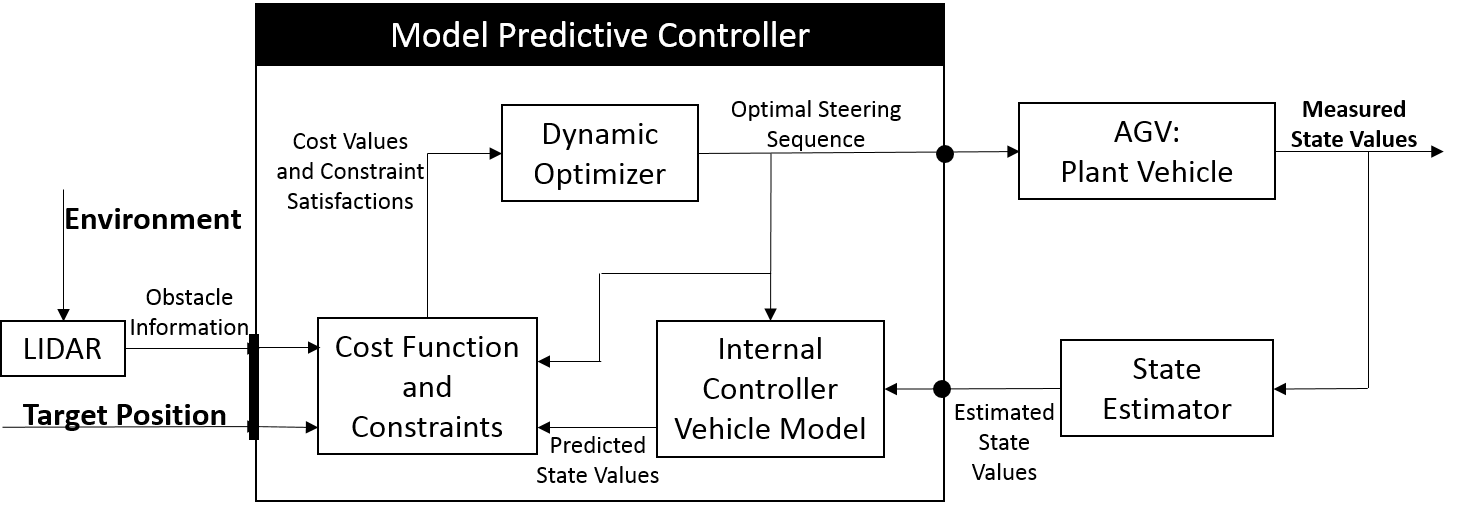
\includegraphics[width=\columnwidth]{Figs/MPCBlockDiagram.png}
	\caption{\small Schematic of MPC LIDAR-Based Constant Speed Local Obstacle Avoidance Controller.  \todo[inline]{adjust sizing of schematic text}}    
	\label{fig:MPC_schematic}
\end{figure}

The planar LIDAR sensor is mounted at the front center location of the vehicle. The LIDAR sensor returns the closest obstacle boundary in all radial directions of the sensor at an angular resolution ε. The LIDAR sensor has a maximum range past which it cannot sense any obstacles. Therefore, if the closest obstacle boundary is greater than the LIDAR radius $R_{LIDAR}$ then the sensor returns $R_{LIDAR}$. The LIDAR sensor range is [0$^o$,180$^o$] with 90$^o$ being the vehicle heading direction. Since for this study the AGV is driving along level ground, whether granular or rigid, the planar LIDAR sensor is sufficient. The LIDAR is assumed to have no delay and zero noise. Therefore, the LIDAR sensor can instantaneously generate a safe area polygon assembled from the returned points from the LIDAR. An overhead view of the AGV encountering an obstacle and the generated LIDAR safe area polygon are presented in Fig.~\ref{fig:obstacle_field}. 
%
\begin{figure}
	\centering
	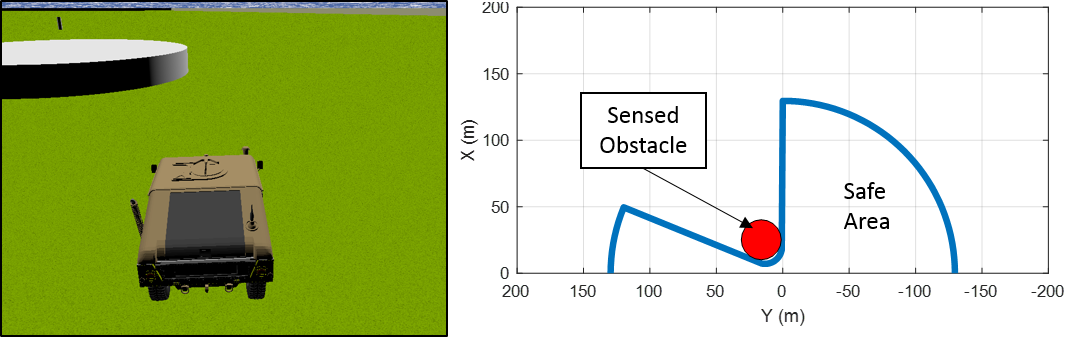
\includegraphics[width=\columnwidth]{Figs/LIDARExample.png}
	\caption{\small Sample obstacle field and LIDAR output.}    
	\label{fig:obstacle_field}
\end{figure}
	
The outputs of the MPC algorithm are the steering signals only for this simulation. As shown in Fig.~\ref{fig:MPC_schematic}, the MPC algorithm is made up of the internal controller vehicle model, the cost function and constraints, and the dynamic optimizer. The internal controller vehicle model predicts the future states of the AGV for a given steering sequence and is of interest in this work. For this study, the internal controller vehicle model is varied from test to test between a 2-DOF vehicle model and a 14-DOF vehicle model, detailed in further sections. The cost functions and constraints are used to formulate the optimal control problem with the equations from the vehicle model. The dynamic optimizer then solves the optimal control problem. For the purpose of this paper, exhaustive search is used to find the optimal solution to the problem since solution speed is not a primary focus of this paper, but more importantly the ability to find and execute an optimal solution.

The same controller as formulated in~\cite{ModelFidelity2016} is used for this study. The cost function and constraints need to be specified to avoid collisions with obstacles and guarantee vehicle dynamical safety. The optimal control problem solved at each MPC time step is comprised of the following set of equations:

\begin{equation}\label{e:MPCCost}
J = s_T + wd 
\end{equation}
\begin{equation}\label{e:State_ODE}
\dot{\xi} = v\left[\xi\left(t\right),\zeta\left(t\right)\right] 
\end{equation}
\begin{equation}\label{e:InitialStates}
\xi\left(0\right) = \xi_0 
\end{equation}
\begin{equation}\label{e:SafeArea}
\tilde{S}\left[x\left(t\right),y\left(t\right)\right] \leq0  
\end{equation}
\begin{equation}\label{e:SteerLimit}
\left|\delta_f\left(t\right)\right| \leq\tilde{\delta}_{f,max}\left(U_0\right) 
\end{equation}
\begin{equation}\label{e:SteerRateLimit}
\left|\varsigma_f\left(t\right)\right| \leq\varsigma_{f,max} 
\end{equation}
\begin{equation}\label{e:TimeDomain}
t \in \left[0,T_P\right]
\end{equation}

Equation~(\ref{e:MPCCost}) defines the cost function for this optimal control problem. This equation is a soft requirement which defines how the separate path possibilities are weighed against each other and how to determine which path is actually optimal. The cost function is comprised of two terms defined by the following
%
\begin{equation}\label{e:DistanceCost}
s_T = \sqrt{\left[ x_G - x\left(T_P\right)\right]^2 + \left[y_G - y\left(T_P\right)\right]^2 }
\end{equation}
\begin{equation}\label{e:TurningCost}
d = \int \limits_0^{T_G} \left|\varsigma\left(t\right)\right| dt 
\end{equation}
%
$s_{T}$ seeks to minimize the distance between the prediction end location and the target position. Refer to \todo{Figure XX} for a visualization of this magnitude. A prediction path that predicts the vehicle at the closest location to the target will have the smaller $s_{T}$ term. The second term $d$ aims to minimize the change in steering angle so that smoother, straighter paths are more favorable than windy paths.

Equations~(\ref{e:State_ODE}-\ref{e:TimeDomain}) are the constraint equations for this optimal control problem which represent hard requirements for vehicle safety and avoiding collisions. Any paths that violate these constraints are not considered safe paths and are eliminated as potential options in this prediction window. Equation~(\ref{e:State_ODE}) defines a set of differential equations that describe the internal controller vehicle model. These equations are presented further in the paper or left for formulation in references. Equation~(\ref{e:InitialStates}) presents the initial states needed to solve Eq.~(\ref{e:State_ODE}) for potential paths. 

Equation~(\ref{e:SafeArea}) defines a safe area polygon. All points along paths found from Eqs.~(\ref{e:State_ODE})-(\ref{e:InitialStates}) must fall inside of this safe area polygon. This safe area is constructed from LIDAR points. An additional safety buffer is added to account for vehicle size and prevent corners of the vehicle from colliding with an obstacle. 

Equation~(\ref{e:SteerLimit}) imposes a limit on maximum steering angle for the vehicle based on vehicle speed. This value is obtained from a lookup table which can be generated either experimentally or from simulation. Equation~(\ref{e:SteerRateLimit}) imposes a maximum limit on steering rate. Equation~(\ref{e:TimeDomain}) defines the time limits over which this optimal control problem is solved.

Equation ~(\ref{e:State_ODE}) as noted above refers to an analytical vehicle model expressed as a set of differential equations. This is how the controller is able to predict vehicle performance within the prediction horizon. The accuracy of the internal vehicle controller model should directly influence the driven vehicle's controlled performance. If the internal vehicle controller model poorly predicts a vehicle's response to inputs from the driver or the environment, then these deficciencies will be witnessed when attempting to control the driven vehicle. In the case of this study, an internal vehicle controller model that poorly represents the driven vehicle may predict that a specified steering sequence will navigate the driven vehicle around an approaching obstacle, but due to this descrepancy the driven vehicle may not turn quickly enough and collide with the obstacle. However, using an internal vehicle controller model that is highly complex may provide accurate trajectory and vehicle response predictions, but the time required to solve an optimal control problem with this complicated set of differential equations is much higher than using a simpler internal vehicle controller model. Since the eventual goal is physical implementation of this controller, an ideal controller would not just accurately predict vehicle responses but also do it quick enough to insure vehicle safety. Therefore for this study the driven vehicle that will be controlled is a HMMWV developed in {\CHRONO}. This vehicle will be controlled using two separately developed controllers. The first controller uses a simple 2 DOF vehicle model to predict the {\CHRONO}  HMMWV trajectory for different series of steering sequences and is presented in detail in Section~\ref{sss:2DOFModel}. The second controller uses a complex 14 DOF vehicle model to predict vehicle states for different series of steering sequences. Once again, this study will test each of these controller's abilities to successfully navigate the driven {\CHRONO}  HMMWV vehicle through two obstacle fields on rigid flat terrain and then granular terrain. The driven {\CHRONO} HMMWV vehicle is presented in detail in Section~\ref{ss:FullVehicleModel}. Exhaustive search space is used to solve the optimal control problem in each time step since the goal of this study is to analyze the vehicle's ability to be successfully navigated through an obstacle field and not how quickly the problem can be solved. A sample visualization of the different predicted trajectories from the 2 DOF model is presented in Fig.~\ref{fig:PossiblePaths}. A point in polygon algorithm is used to determine which trajectories remain inside of the safe area polygon and therefore should be compared to the other possibilities using Eq.~(\ref{e:MPCCost}).

\begin{figure}
	\centering
	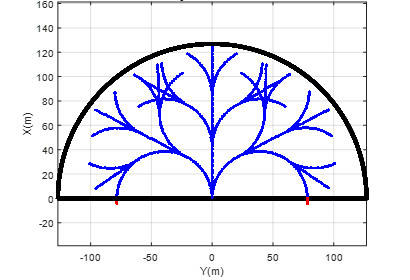
\includegraphics[width=\columnwidth]{Figs/PathPossibilities.png}
	\caption{\small Potential Paths predicted by 2 DOF Internal Vehicle Controller Model}  
	\label{fig:PossiblePaths}
\end{figure}

%% ============================================================

\subsection{{\CHRONO} Multibody Physics Package}\label{ss:Chrono}

The physics modeling and simulation capabilities are provided by the multiphysics open-source package {\CHRONO}~\cite{Chrono2016}. The core functionality of {\CHRONO} provides support for the modeling, simulation, and visualization of rigid multibody systems, with additional capabilities offered through optional modules. These modules provide support for additional classes of problems (e.g., finite element analysis and fluid-solid interaction), for modeling and simulation of specialized systems (such as ground vehicles and granular dynamics problems), or provide specialized parallel computing algorithms (multi-core, GPU, and distributed) for large-scale simulations.

\todo[inline]{More about Chrono: design, availability, existing modules.\\Short description of Chrono::Parallel}

%% ------------------------------------------------------------

\subsubsection{Vehicle Modeling}\label{sss:Chrono_Vehicle}
	
Built as a {\CHRONO} extension module, {\ChronoVehicle}~\cite{TR2016-10RaduChronoVehicle} is a C++ middleware library focused on the modeling, simulation, and visualization of ground vehicles.
%
{\ChronoVehicle} provides a collection of templates for various topologies of both wheeled and tracked vehicle subsystems, as well as support for modeling of rigid, flexible, and granular terrain, support for closed-loop and interactive driver models, and run-time and off-line visualization of simulation results.


\todo[inline]{More about Chrono::Vehicle (template-based design, supported topologies, driver models)...}

%% ------------------------------------------------------------

\subsubsection{Granular Mechanics }\label{sss:GranMech}

In this work, the focus is on modeling and simulating the terrain and the tire-terrain interaction using high-fidelity, fully-resolved granular dynamics simulations, employing the so-called Discrete element Method (DEM).  Meaningful mobility simulations require large enough terrain patches and small enough particle dimensions that result in DEM problems involving frictional contact with millions of degrees of freedom.

\todo[inline]{More about DEM (NSC and SMC)...}

%%============================================================

\section{TECHNICAL APPROACH AND METHODOLOGY}\label{s:methodology}

\subsection{Chrono Full-Vehicle Model to be Controlled}\label{ss:FullVehicleModel}

\todo[inline]{Description of the HMMWV Chrono::Vehicle model used as the plant}

%% ============================================================

\subsection{Relocating Granular Patch }\label{ss:Patch}

%% ============================================================

\subsection{Internal Controller Vehicle Models}\label{ss:IntModel}

The vehicle models embedded in the MPC are simplifications of the full, multi-body based, {\CHRONO} wheeled vehicle model which is being controlled.  We consider two such models, providing different levels of fidelity, as described below.

%% ------------------------------------------------------------

\subsubsection{Two DOF Vehicle Model}\label{sss:2DOFModel}
The standard vehicle model used in newly developed MPC obstacle avoidance algorithms such as~\cite{ModelFidelity2016} is the 2-DOF vehicle model. These models normally either assume constant cornering stiffness or the nonlinear Pacejka Magic Formula Tire Model~\cite{foo} to predict the ground tire interaction forces. For this study and due to the availability of experimental data, the Pacejka Magic Formula is used to predict tire forces in the vehicle models.   

\begin{figure}
	\centering
	
\includegraphics[width=\columnwidth]{Figs/no-image.png}
	\caption{\small Two DOF Vehicle Model}  
	\label{fig:2DOF}
\end{figure}

A visual representation of the 2-DOF model can be found in Fig.~\ref{fig:2DOF}. The two DOF model is described by the following first-order ordinary differential equations:

\begin{equation}\label{e:2DOF_Vdot}
\dot{V} = \left(F_{y,f} + F_{y,r}\right)/{M - U_0r} 
\end{equation}
\begin{equation}\label{e:2DOF_rdot}
\dot{r} = \left(F_{y,f} - F_{y,r}\right)/I_{zz}
\end{equation}
\begin{equation}\label{e:2DOF_psidot}
\dot{\psi} = r 
\end{equation}
\begin{equation}\label{e:2DOF_xdot}
\dot{x} = U_0\cos{\psi}-\left(V+L_fr\right)\sin{\psi}
\end{equation}
\begin{equation}\label{e:2DOF_ydot}
\dot{y} = U_0\sin{\psi}+\left(V+L_fr\right)\cos{\psi} \,,
\end{equation}
%
where $F_{y,f}$ and $F_{y,r}$ are the lateral tire forces at the front and rear axles, respectively. $U_0$ and $V$ are the longitudinal speed and lateral speed of the vehicle in the vehicle’s coordinate frame. $\psi$ is the yaw angle and $r$ is the yaw rate. $\left(x,y\right)$ represent the front center location of the vehicle expressed in global coordinates. $M$ is vehicle mass, $I_{zz}$ is the moment of inertia of the vehicle, $L_f$ is the distance from the front axle to the vehicle CoG, and $L_r$ is the distance from the rear axle to the vehicle CoG.
\todo[inline]{ Add more here }


%% ------------------------------------------------------------

\subsubsection{Fourteen DOF Vehicle Model}\label{sss:14DOFModel}
A fourteen DOF model is often used in studies such as these to test the obstacle avoidance controller with a higher fidelity vehicle model~\cite{ModelFidelity2016, ModelFidelity2013}. A benefit of using the fourteen DOF in the controller is the model’s ability to predict tire liftoff and account for dynamic effects from suspension systems. For this paper then it is appropriate to also compare performance of the local obstacle avoidance controller running an internal fourteen DOF on rigid terrain versus granular terrain.  

The fourteen DOF vehicle model consists of one sprung mass connected above four unsprung masses~\cite{RollStudies2007}. A visual representation of the fourteen DOF vehicle model can be found in Fig.~\ref{fig:14DOF}. The sprung mass is allowed to roll, pitch, and yaw while also displacing laterally, vertically, and longitudinally. This sprung mass contributes six DOF to the model. Each of the four wheels are allowed to bounce vertically and rotate about the wheel horizontal axis. The front two wheels are also free to steer. Each wheel then contributes two DOF to the fourteen DOF model. The equations used for this model as well as their developments can be found in~\cite{RollStudies2007}.

\begin{figure}
	\centering
	
\includegraphics[width=\columnwidth]{Figs/no-image.png}
	\caption{\small Fourteen DOF Vehicle Model}  
	\label{fig:14DOF}
\end{figure}

The Pacejka Magic Formula is used to calculate the ground tire interaction forces in the fourteen DOF vehicle model. On rigid terrain, this is an accurate and valid assumption. However, based on how the Pacejka Magic Formula is derived and coefficients experimentally obtained, using the Magic Formula to estimate tire forces on granular terrain is not a valid assumption. However, this estimation may provide tire forces that are close enough to still allow the vehicle to successfully navigate the obstacle field safely. 
\todo[inline]{ finish this paragraph}
\todo[inline] {Add 14DOF vehicle model figure}

%% ============================================================
\subsection{Open Loop Comparisons }\label{ss:OpenLoop}

%% ============================================================

\subsection{Evaluation Metrics}\label{ss:Metrics}
Five evaluation metrics will be used to compare one test performance to the other. First, all test runs will be compared based on the time to reach the target $T_{target}$. Tests on the same terrain can be compared with this metric to determine which controller leads the vehicle to the target point quickest. Second, the closest distance the vehicle reaches to any obstacle $d_{min}$ will be measured. A controller that accurately predicts vehicle performance should allow the vehicle get much closer to obstacles. Third, the control effort will be calculated and compared between test cases. Fourth, the max lateral acceleration of the vehicle will be determined. Finally, the average lateral acceleration will be determined from the test cases. These five evaluation metrics provide a logical method for comparing one test case to another whether two test cases are on different terrain, have different analytical controller models, or both. 

%% ============================================================

\subsection{Numerical Simulation Setup }\label{ss:Setup}
Simulations on both rigid and granular terrain were compared to understand how the controller performs on non-ideal surfaces.  The two internal controller vehicle models to be studied in these tests are the previously described two DOF and fourteen DOF vehicle models. Aside from changing the internal controller vehicle model from study to study, the rest of the controller will remain the same. Referring to Table~\ref{t:TestMatrix}, Tests 1 and 2 will be compared to understand how model fidelity influences controller performance on rigid flat terrain. Tests 3 and 4 will be compared to again understand the role of model fidelity in the MPC controller on granular terrain. Tests 1 and 3 will be compared to understand how the same controller performs differently on granular terrain as opposed to rigid flat terrain. Similar comparisons will be made between Tests 2 and 4. Each of the tests will consist of one run on two different obstacle fields created to target the controller’s ability to navigate the vehicle through certain obstacle combinations.

\begin{table}
\begin{center}
	\begin{tabular}{||c |c | c||} 
		\hline
		Test  & Terrain  & Controller Vehicle \\
		Number &  Type & Model\\ [0.5ex] 	
		\hline\hline
		1 & Rigid & 2DOF \\ 
		\hline
		2 & Rigid & 14DOF \\
		\hline
		3 & Granular & 2DOF \\
		\hline
		4 & Granular & 14DOF \\
		\hline
	\end{tabular}
\end{center}
\caption{Individual Simulation Test Information}
\label{t:TestMatrix}
\end{table}

For this paper two obstacle fields were generated. The first contains one large circular obstacle located along the initial heading of the vehicle. The target position is located a large distance then behind the single obstacle. Figure~\ref{f:Obst1} presents this obstacle field. The goal of this test is to analyze the performance of the vehicle and controller around a single obstacle. 

The second obstacle field contains four circular obstacles of varying sizes placed in the vehicle’s initial heading direction. The performance of the vehicle on this obstacle field should allow for understanding of how the controller and vehicle navigate around multiple obstacles in a more realistic scenario. Refer to Fig.~\ref{f:Obst2}.

\begin{figure}
	\centering
	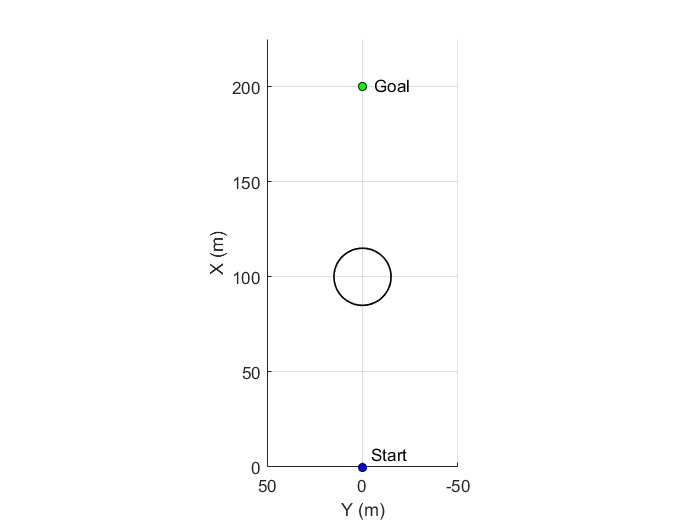
\includegraphics[width=\columnwidth]{Figs/ObstacleField1.png}
	\caption{\small Obstacle Field 1}  
	\label{fig:Obst1}
\end{figure}

\begin{table}
\begin{center}
	\begin{tabular}{||c|c|c|c||} 
		\hline
		& x & y & Radius\\
		\hline
		Target Location  & 200.0 & 0.0 & -\\ 
		\hline
		Obstacle 1 & 100.0 & 0.0 & 15.0\\
		\hline
	\end{tabular}
\end{center}
\caption{Obstacle Field 1 Summary}
\label{t:Obst1Summary}
\end{table}

\begin{figure}
	\centering
	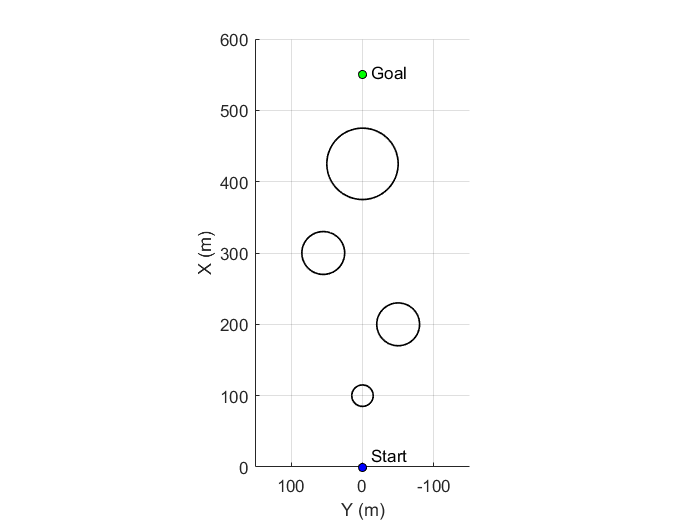
\includegraphics[width=\columnwidth]{Figs/ObstacleField2.png}
	\caption{\small Obstacle Field 2}   
	\label{fig:Obst2}
\end{figure}

\begin{table}
\begin{center}
	\begin{tabular}{||c|c|c|c||} 
		\hline
		& x & y & Radius\\
		\hline
		Target Location  & 550.0 & 0.0 & -\\ 
		\hline
		Obstacle 1 & 100.0 & 0.0 & 15.0\\
		\hline
		Obstacle 2 & 200.0 & -50.0 & 30.0\\
		\hline
		Obstacle 3 & 300.0 & 55.0 & 30.0\\
		\hline
		Obstacle 4 & 425.0 & 0.0 & 50.0\\
		\hline
	\end{tabular}
\end{center}
\caption{Obstacle Field 2 Summary}
\label{t:Obst2Summary}
\end{table}

%% ============================================================

\section{SIMULATION RESULTS}\label{s:results}

%% ============================================================

\subsection{Test Results}\label{ss:test_results}
This section summarizes the results of the four tests listed in Table~\ref{t:TestMatrix}.

\subsubsection{Test 1 Results}\label{sss:Test1}

\begin{figure}
	\centering
	
\includegraphics[width=\columnwidth]{Figs/no-image.png}
	\caption{\small Test 1 Vehicle Trajectory Obstacle Field 1}  
	\label{fig:Test1_Obst1}
\end{figure}

\begin{figure}
	\centering
	
\includegraphics[width=\columnwidth]{Figs/no-image.png}
	\caption{\small Test 1 Obstacle Field 1 Steering Commands}  
	\label{fig:Test1_Obst1_Steer}
\end{figure}

\begin{table}
\begin{center}
	\begin{tabular}{||c |c||} 
		\hline
		$T_{target}$ & ??\\ 
		\hline
		$d_{min}$ & ??\\
		\hline
		Control Effort & ??\\
		\hline
		Max Lateral Acceleration & ??\\
		\hline
		Avg. Lateral Acceleration & ??\\
		\hline
	\end{tabular}
\end{center}
\caption{Evaluation Metrics Test 1 Obstacle Field 1}
\label{t:EvalTest1Obst1}
\end{table}

\begin{figure}
	\centering
	
\includegraphics[width=\columnwidth]{Figs/no-image.png}
	\caption{\small Test 1 Vehicle Trajectory Obstacle Field 2}  
	\label{fig:Test1_Obst2}
\end{figure}

\begin{figure}
	\centering
	
\includegraphics[width=\columnwidth]{Figs/no-image.png}
	\caption{\small Test 1 Obstacle Field 2 Steering Commands}  
	\label{fig:Test1_Obst2_Steer}
\end{figure}

\begin{table}
\begin{center}
	\begin{tabular}{||c |c||} 
		\hline
		$T_{target}$ & ??\\ 
		\hline
		$d_{min}$ & ??\\
		\hline
		Control Effort & ??\\
		\hline
		Max Lateral Acceleration & ??\\
		\hline
		Avg. Lateral Acceleration & ??\\
		\hline
	\end{tabular}
\end{center}
\caption{Evaluation Metrics Test 1 Obstacle Field 2}
\label{t:EvalTest1Obst2}
\end{table}
%% ------------------------------------------------------------

\subsubsection{Test 2 Results}\label{sss:Test2}

\begin{figure}
	\centering
	
\includegraphics[width=\columnwidth]{Figs/no-image.png}
	\caption{\small Test 2 Vehicle Trajectory Obstacle Field 1}  
	\label{fig:Test2_Obst1}
\end{figure}

\begin{figure}
	\centering
	
\includegraphics[width=\columnwidth]{Figs/no-image.png}
	\caption{\small Test 2 Obstacle Field 1 Steering Commands}  
	\label{fig:Test2_Obst1_Steer}
\end{figure}

\begin{table}
\begin{center}
	\begin{tabular}{||c |c||} 
		\hline
		$T_{target}$ & ??\\ 
		\hline
		$d_{min}$ & ??\\
		\hline
		Control Effort & ??\\
		\hline
		Max Lateral Acceleration & ??\\
		\hline
		Avg. Lateral Acceleration & ??\\
		\hline
	\end{tabular}
\end{center}
\caption{Evaluation Metrics Test 2 Obstacle Field 1}
\label{t:EvalTest2Obst1}
\end{table}

\begin{figure}
	\centering
	
\includegraphics[width=\columnwidth]{Figs/no-image.png}
	\caption{\small Test 2 Vehicle Trajectory Obstacle Field 2}  
	\label{fig:Test2_Obst2}
\end{figure}

\begin{figure}
	\centering
	
\includegraphics[width=\columnwidth]{Figs/no-image.png}
	\caption{\small Test 2 Obstacle Field 2 Steering Commands}  
	\label{fig:Test2_Obst2_Steer}
\end{figure}

\begin{table}
\begin{center}
	\begin{tabular}{||c |c||} 
		\hline
		$T_{target}$ & ??\\ 
		\hline
		$d_{min}$ & ??\\
		\hline
		Control Effort & ??\\
		\hline
		Max Lateral Acceleration & ??\\
		\hline
		Avg. Lateral Acceleration & ??\\
		\hline
	\end{tabular}
\end{center}
\caption{Evaluation Metrics Test 2 Obstacle Field 2}
\label{t:EvalTest2Obst2}
\end{table}

%% ------------------------------------------------------------

\subsubsection{Test 3 Results}\label{sss:Test3}

\begin{figure}
	\centering
	
\includegraphics[width=\columnwidth]{Figs/no-image.png}
	\caption{\small Test 3 Vehicle Trajectory Obstacle Field 1}  
	\label{fig:Test3_Obst1}
\end{figure}

\begin{figure}
	\centering
	
\includegraphics[width=\columnwidth]{Figs/no-image.png}
	\caption{\small Test 3 Obstacle Field 1 Steering Commands}  
	\label{fig:Test3_Obst1_Steer}
\end{figure}

\begin{table}
\begin{center}
	\begin{tabular}{||c |c||} 
		\hline
		$T_{target}$ & ??\\ 
		\hline
		$d_{min}$ & ??\\
		\hline
		Control Effort & ??\\
		\hline
		Max Lateral Acceleration & ??\\
		\hline
		Avg. Lateral Acceleration & ??\\
		\hline
	\end{tabular}
\end{center}
\caption{Evaluation Metrics Test 3 Obstacle Field 1}
\label{t:EvalTest3Obst1}
\end{table}

\begin{figure}
	\centering
	
\includegraphics[width=\columnwidth]{Figs/no-image.png}
	\caption{\small Test 3 Vehicle Trajectory Obstacle Field 2}  
	\label{fig:Test3_Obst2}
\end{figure}

\begin{figure}
	\centering
	
\includegraphics[width=\columnwidth]{Figs/no-image.png}
	\caption{\small Test 3 Obstacle Field 2 Steering Commands}  
	\label{fig:Test3_Obst2_Steer}
\end{figure}
\begin{table}
\begin{center}
	\begin{tabular}{||c |c||} 
		\hline
		$T_{target}$ & ??\\ 
		\hline
		$d_{min}$ & ??\\
		\hline
		Control Effort & ??\\
		\hline
		Max Lateral Acceleration & ??\\
		\hline
		Avg. Lateral Acceleration & ??\\
		\hline
	\end{tabular}
\end{center}
\caption{Evaluation Metrics Test 3 Obstacle Field 2}
\label{t:EvalTest3Obst2}
\end{table}

%% ------------------------------------------------------------

\subsubsection{Test 4 Results}\label{sss:Test4}

\begin{figure}
	\centering
	
\includegraphics[width=\columnwidth]{Figs/no-image.png}
	\caption{\small Test 4 Vehicle Trajectory Obstacle Field 1}  
	\label{fig:Test4_Obst1}
\end{figure}

\begin{figure}
	\centering
	
\includegraphics[width=\columnwidth]{Figs/no-image.png}
	\caption{\small Test 4 Obstacle Field 1 Steering Commands}  
	\label{fig:Test4_Obst1_Steer}
\end{figure}

\begin{table}
\begin{center}
	\begin{tabular}{||c |c||} 
		\hline
		$T_{target}$ & ??\\ 
		\hline
		$d_{min}$ & ??\\
		\hline
		Control Effort & ??\\
		\hline
		Max Lateral Acceleration & ??\\
		\hline
		Avg. Lateral Acceleration & ??\\
		\hline
	\end{tabular}
\end{center}
\caption{Evaluation Metrics Test 4 Obstacle Field 1}
\label{t:EvalTest4Obst1}
\end{table}

\begin{figure}
	\centering
	
\includegraphics[width=\columnwidth]{Figs/no-image.png}
	\caption{\small Test 4 Vehicle Trajectory Obstacle Field 2}  
	\label{fig:Test4_Obst2}
\end{figure}

\begin{figure}
	\centering
	
\includegraphics[width=\columnwidth]{Figs/no-image.png}
	\caption{\small Test 4 Obstacle Field 2 Steering Commands}  
	\label{fig:Test4_Obst2_Steer}
\end{figure}

\begin{table}
\begin{center}
	\begin{tabular}{||c |c||} 
		\hline
		$T_{target}$ & ??\\ 
		\hline
		$d_{min}$ & ??\\
		\hline
		Control Effort & ??\\
		\hline
		Max Lateral Acceleration & ??\\
		\hline
		Avg. Lateral Acceleration & ??\\
		\hline
	\end{tabular}
\end{center}
\caption{Evaluation Metrics Test 4 Obstacle Field 2}
\label{t:EvalTest4Obst2}
\end{table}

%% ============================================================

\subsection{Method Comparisons}\label{ss:comparisons}

To gauge the efficacy and appropriateness of the 2-DOF and 14-DOF models as embedded MPC models, we compare results obtained with each of them on both rigid and granular terrain.  These findings are summarized below.

%% ------------------------------------------------------------

\subsubsection{2-DOF vs. 14-DOF Controllers on Rigid Terrain }\label{sss:Comp1}

%% ------------------------------------------------------------

\subsubsection{2-DOF vs. 14-DOF Controllers on Granular Terrain }\label{sss:Comp2}

%% ------------------------------------------------------------

\subsubsection{2-DOF Controller on Rigid vs. Granular Terrain}\label{sss:Comp3}

%% ------------------------------------------------------------

\subsubsection{14-DOF Controller on Rigid vs. Granular Terrain }\label{sss:Comp4}

%% ============================================================

\section{CONCLUSIONS}\label{s:conclusion}


%% ============================================================

\section*{Acknowledgments}
Support for this research...

%% ============================================================

\bibliographystyle{unsrt}
\bibliography{references}

%% ============================================================


\end{document}



